% THIS IS SIGPROC-SP.TEX - VERSION 3.1
% WORKS WITH V3.2SP OF ACM_PROC_ARTICLE-SP.CLS
% APRIL 2009
%
% It is an example file showing how to use the 'acm_proc_article-sp.cls' V3.2SP
% LaTeX2e document class file for Conference Proceedings submissions.
% ----------------------------------------------------------------------------------------------------------------
% This .tex file (and associated .cls V3.2SP) *DOES NOT* produce:
%       1) The Permission Statement
%       2) The Conference (location) Info information
%       3) The Copyright Line with ACM data
%       4) Page numbering
% ---------------------------------------------------------------------------------------------------------------
% It is an example which *does* use the .bib file (from which the .bbl file
% is produced).
% REMEMBER HOWEVER: After having produced the .bbl file,
% and prior to final submission,
% you need to 'insert'  your .bbl file into your source .tex file so as to provide
% ONE 'self-contained' source file.
%
% Questions regarding SIGS should be sent to
% Adrienne Griscti ---> griscti@acm.org
%
% Questions/suggestions regarding the guidelines, .tex and .cls files, etc. to
% Gerald Murray ---> murray@hq.acm.org
%
% For tracking purposes - this is V3.1SP - APRIL 2009

\documentclass[12pt, letterpaper]{article}
\usepackage{graphicx}
%\graphicspath{ {/analytics/} }
\usepackage{listings}
\usepackage[export]{adjustbox}
\usepackage[utf8]{inputenc}
\setlength{\parindent}{2em}


\title{Kubernetes \& Containers}
\author{Bruce Walker}

%\affaddr{Phoenix, AZ}
%\email{brucwalk@iu.edu}
 
\date{ April 27, 2018}

\begin{document}

\maketitle 

\section*{Introduction}
\setlength{\parskip}{1em}
\indent 
Kubernetes is fast becoming the most influential cloud platform that
many have never heard of.  A recent development, it features power and
flexibility to ensure a place in the future of cloud computing.  It is
a robust collection of processes, that are fast and dependable.  It is
scaleable and adaptive. Kubernetes is a command line application, that
can have GUI characteristics attached.  It essentially uses API's to
describe and manage what applications are running in a container.
\cite {hid-sp18-525-concept}

\section *{How it Works}
\setlength{\parskip}{1.3em}

Developed by Google, Kubernetes is a relatively new technology.  It
started in 2014 as an open source method of deploying and operating
application containers.  

Methods of computing and computing applications have moved from large
applications to VM's to containers.  Applications on computers require
large operating systems, that encompass the entire computer and
require that every application be subject to their commands.  Should
the operating system fail, all applications on the computer will also
fail.   

On the virtual machine, Kubernetes is installed by accessing an
outside site, like GitHub, to download the application.  There a
number of options, when it comes to which application to install.
Part of the variation is due to the particular version of virtual
machine used to run Kubernetes.  Also, the use of a more convenient,
and lighter form of Kubernetes, called Minikube is often used for a
virtual machine, such as
Ubuntu. https://kubernetes.io/docs/getting-started-guides/minikube/.
It is a fast download and can access other Kubernetes options and
APIs.  Even though it is local, it can still support \cite {hid-sp18-525-concept}
\begin{itemize}
    \item DNS 
    
    \item NodePorts 
    
    \item ConfigMaps and Secrets 
    
    \item Dashboards, Container 
    
    \item Runtime:  Docker, rkt, and CRI-O 
    
    \item Container Network Interface
    
    \item Ingress  
 \end{itemize}   
 
Once Kubernetes is installed on the virtual machine, it can be
deployed.  Kubernetes must be configured in order to properly deploy
and, for it to accept containers.  Once deployed, containers, with
applications can be layered on top of Kubernetes.  Kubernetes can then
create instances of the application  \cite {hid-sp18-525-concept}.

A cloud based option for available for Kubernetes use.  Cloud
services, such as, IBM, Microsoft Azure, Amazon AWS, etc., have joined
in using Kubernetes due to the reliability and ability to offer a wide
variety of services to customers.   

Since Kubernetes, and thus MiniKube, are similar to stand alone
machines, many aspects of their performance and behavior must be
configured.  Drivers must be imported.  Minikube supports Kubernetes
features, such as DNS, NodePorts, ConfigMaps and Secrets, etc.   

Kubernetes use of REST API's is the cornerstone of all Kubernetes activity.  


\section *{How Kubernetes is Used}
\setlength{\parskip}{1.6em}
Reference:  https://kubernetes.io/docs/tutorials/kubernetes-basics/explore-intro/

Kubernetes has a hierarchical design.  At the lowest level are Pods.
Generally, Pods are where application containers are placed.  Pods are
the smallest units in the Kubernetes universe.  It essentially acts as
a host for application containers.  Pods can be closely linked, where
a single Pod will contain information, and a different Pod will
contain other information.  The Pods may or may not communicate with
each other.  The can be linked via IP addresses, if they need to
communicate.   

The next level of architecture is the Node.  All Pods run on a Node.
The Node is where much of the actual computing occurs.  A Node may be
physically located on a machine or it may be virtual or cloud
based. The Node allocates the resources needed by the Pods on a
machine.  A Node has a minimum level of processes that it must
perform.  It must run the Kubelet, which orchestrates Node and the
highest level, the Master level.  The Node must also run the what is
in the container.  The container application, Docker, for example is
managed by the Node.  It retrieves the container image from the
registry and then opens the application in the container.  Thereafter,
it runs the application. 

The Kubectl is the heart of Pod interactions.  It shows and details
resources and can execute commands and print logs from the Pod. 

Each Pod is a self contained environment, which requires authorization
and or proxy to access.  No alteration of the Pod can take place until
the kubectl proxy command is executed, in a separate terminal window.   
 


Kubernetes is deployed in a number of ways.  That number is
increasing, especially when cloud services are included.  On a local
machine, Kubernetes is deployed on a host machine and or on a virtual
machine, such as Ubuntu.  On the local machine, Kubernetes can be
deployed via the command line, using the following commands: 


On the virtual machine, deployment can occur through VirtualBox or
other VM.  The host operating system may require a BIOS update to
ensure the proper virtualization settings.   

Deploying Kubernetes to support a Docker environment is very popular.
Kubernetes can manage the Docker containers via a Kubernetes Service.
The service establishes policies that manage who has access to Pods.
This is referred to as a microservice.  Kubernetes services ensure a
high, overall level of reliability.  When Pods fail, their functions
are continued by replication controllers ensure that sufficient Pods
are available to perform as needed, without failure.  When a Pod is
created, additional Pods maybe created, identically structured, in
order to ensure availability of Pod functions
\cite{hid-sp18-525-service}.  

\section *{How to Get Started}
\setlength{\parskip}{1.6em}

Kubernetes is able to run on desktop and virtual machines.  In order
to started on a Mac, Kubernetes is installed.  Thereafter, a container
service, such as Docker can be downloaded.  Docker includes an option,
for Mac, that includes Kubernetes.  The two applications compliment
each other  \cite{hid-sp18-525-service}.  

Downloading Kubernetes
\setlength{\parskip}{1.6em}


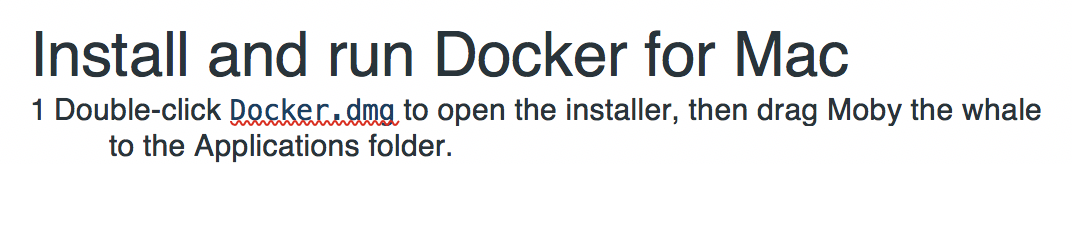
\includegraphics[width=1\textwidth, center]{Install Docker.png}

Kubernetes, and the applications it supports, are easily downloaded.
Upon downloading, Docker can be layered on top of Kubernetes.   

\section *{What can you put in Kubernetes}

Although Docker is loaded onto a local machine, in these examples,
cloud and virtual deployments are also available
\cite{hid-sp18-525-docker}. 

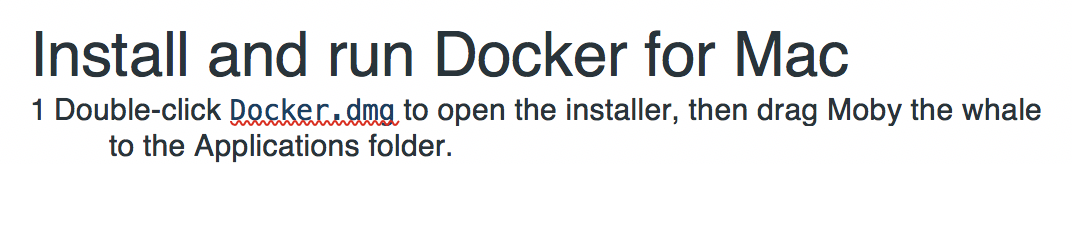
\includegraphics[width=1\textwidth, right]{Install Docker.png}
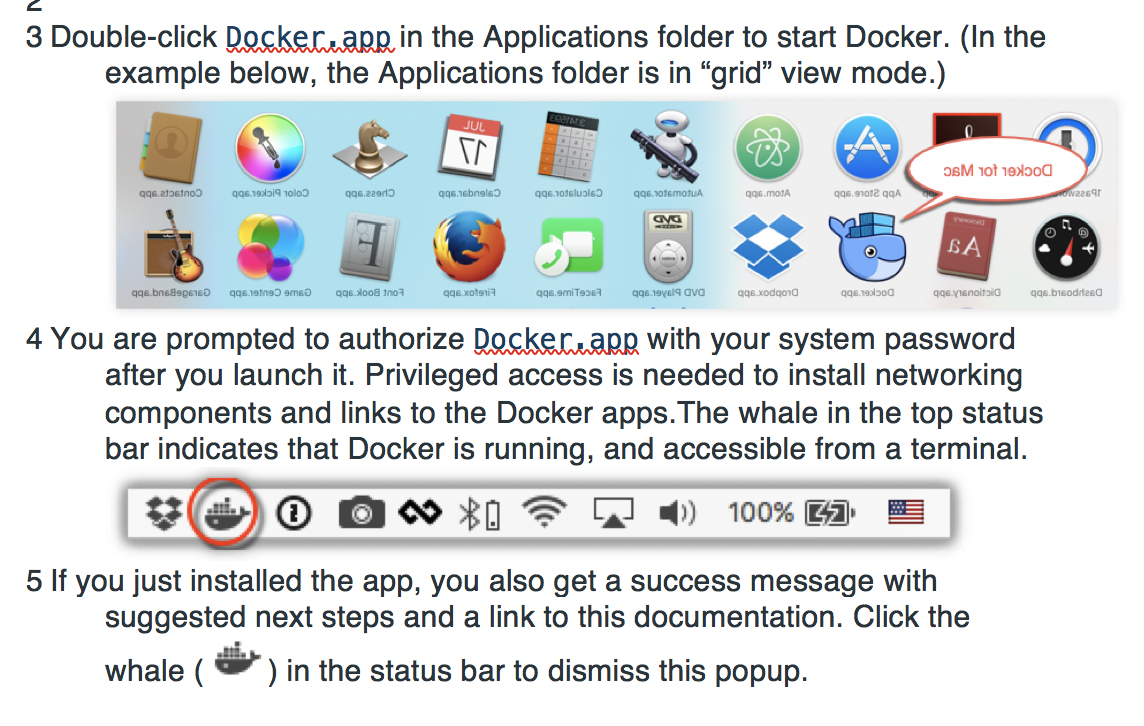
\includegraphics[width=1\textwidth, right]{Install Docker2.png}
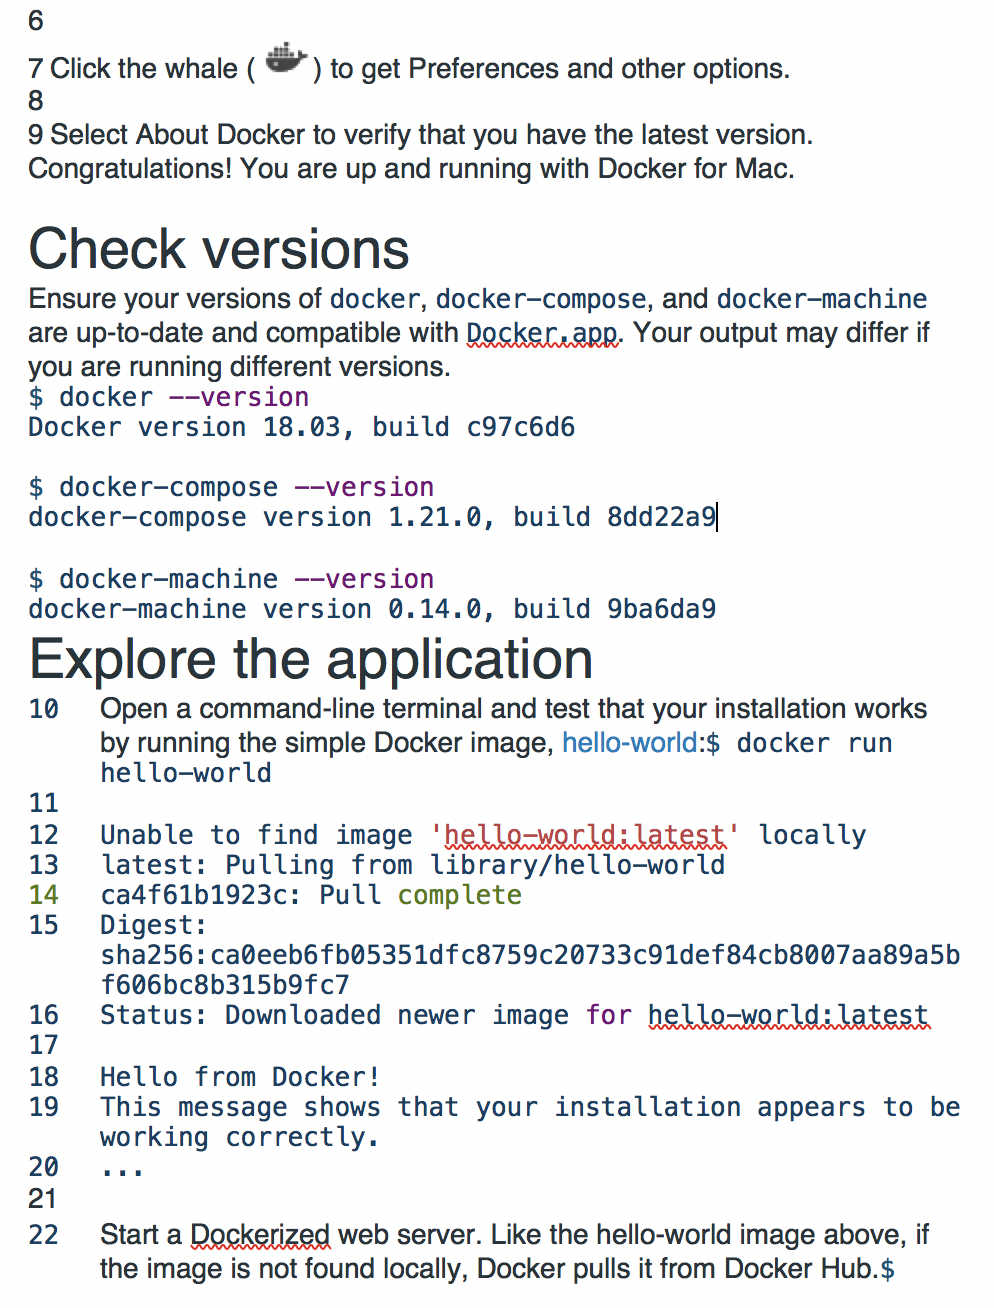
\includegraphics[width=1\textwidth, right]{Install Docker3.png}
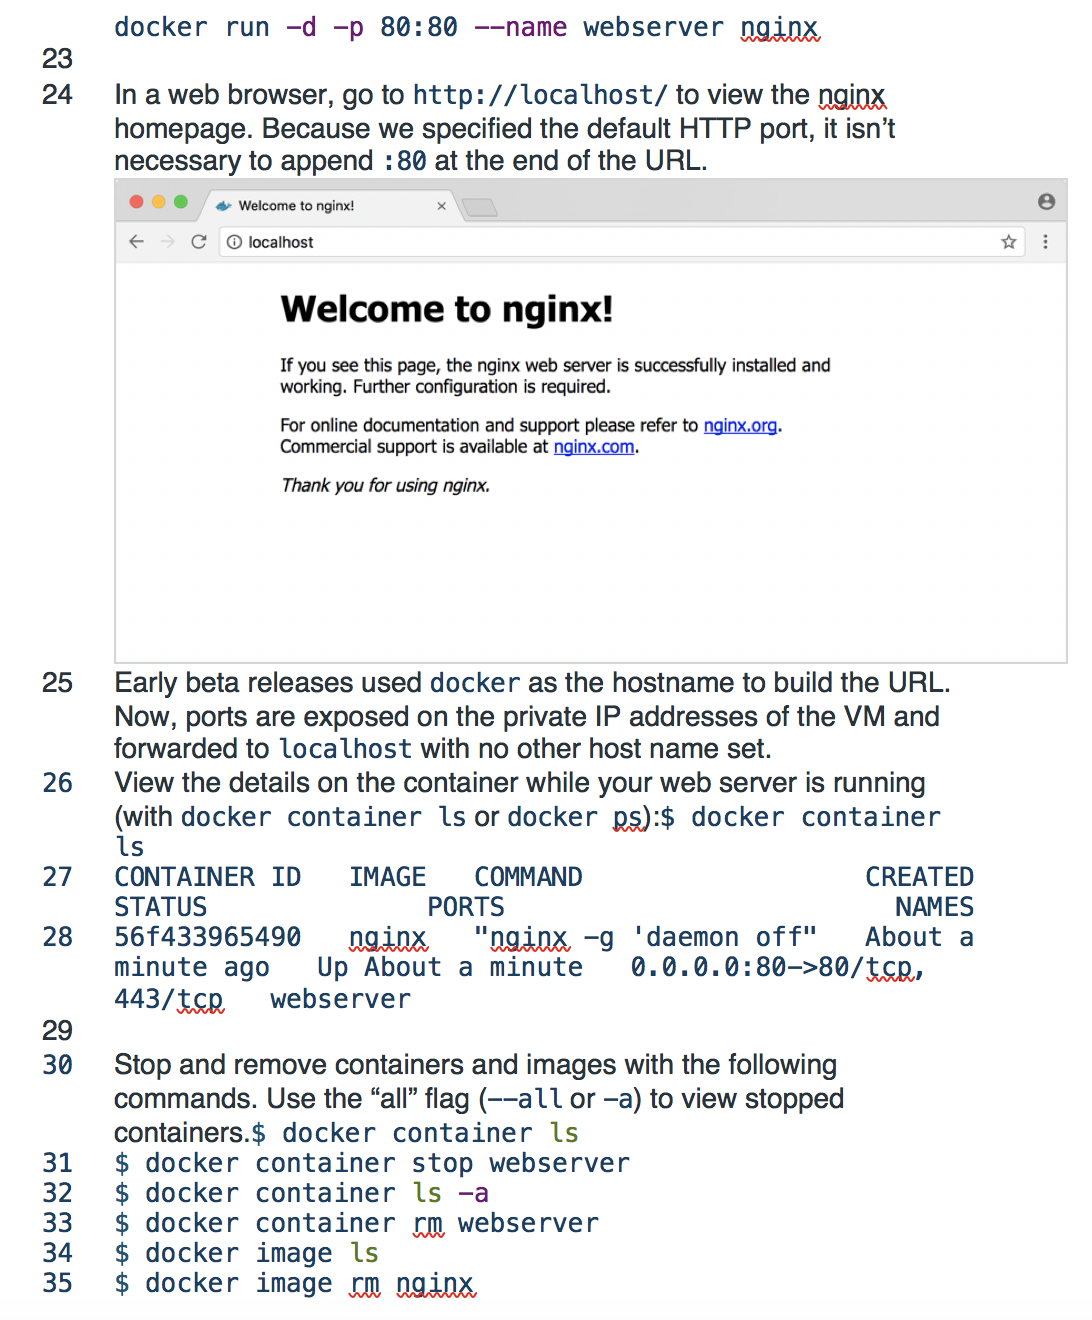
\includegraphics[width=1\textwidth, right]{Install Docker4.png}



\bibliographystyle{article}
\bibliography{hid-sp18-525}



\end{document}
